

\chapter{Understanding Scientific Publications}
\label{ch:sci}

In Chapter~\ref{ch:nonfiction}, we discuss how scholars use topic models to understand
non-fiction documents.  This chapter focuses on a particular sub-genre of
non-fiction: scientific documents.  Scientific documents deserve their own
chapter because these documents are unique: they use very specialized
vocabulary, they are the vehicles for innovation, and they shape important
policy decisions.  We discuss each of these aspects in turn.

\begin{figure}
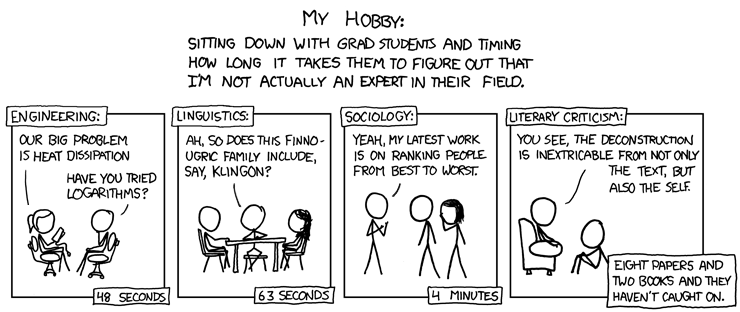
\includegraphics[width=\linewidth]{figures/sci_faking}
\caption{Using the appropriate language is a prerequisite for being
  part of a field (but not sufficient).  Topic models use this to
  automatically discover fields of study.}
\label{fig:faking}
\end{figure}

\paragraph{Specialized Vocabularies Define Fields of Study}

First, scientific documents are unique because unlike general documents,
their vocabulary is precise and carefully measured.  ``Resistance'', ``splice'',
``utilization'', and ``demand'' are common words with radically different
meanings when used in specialized, technical contexts.  Their use is a
marker for membership in a specific discipline
(Figure~\ref{fig:faking}).  Thus, the ability of topic models to capture
patterns of word usage also captures community and affiliation; this goes well
beyond the thematic uses of topic models described in previous chapters.

\paragraph{Scientific Documents Innovate}

Not every scientific publication is innovative;
in fact, most are not.  However, some scientific publications are
Earth-shaking. Such developments might be theoretical, or methodological, or empirical.
Physics was revolutionized by relativity.
Genetics was revolutionized by the discovery of polymerase chain reaction methods. 
Geology was revolutionized by the discovery of evidence for plate tectonics in the form of magnetic traces in the ocean floor. Unlike the other domains we have
discussed, scientific documents are not just \emph{reports} of news or events;
they actually \emph{are the news}.

What makes the analysis of scientific document collections both challenging and
interesting is that innovation is hard to detect and hard to attribute.
Einstein's groundbreaking 1905 papers were not fully recognized until many years
later; important ideas are often proposed by an obscure researcher but only accepted
once popularized and supported by other research. Which document (or researcher)
in this case was the true source of the innovation?  As we will see in this
chapter, topic models can help answer this question.

\paragraph{Science and Policy}

Understanding scientific publications is important for funding agencies,
lawmakers, and the public.  Government funding of science can create jobs,
improve culture, and is an important form of international ``soft power''.
However, knowing which research to fund is difficult, as the nature of science
means that fields constantly change, which precludes rigid
classifications~\citep{szostak-04}.  One challenge of modeling scientific
documents is modeling how fields change over time; the static models we have
discussed thus far are not always appropriate.

\section{Understanding Fields of Studies}
\label{sec:sci_fields}

\begin{figure}
  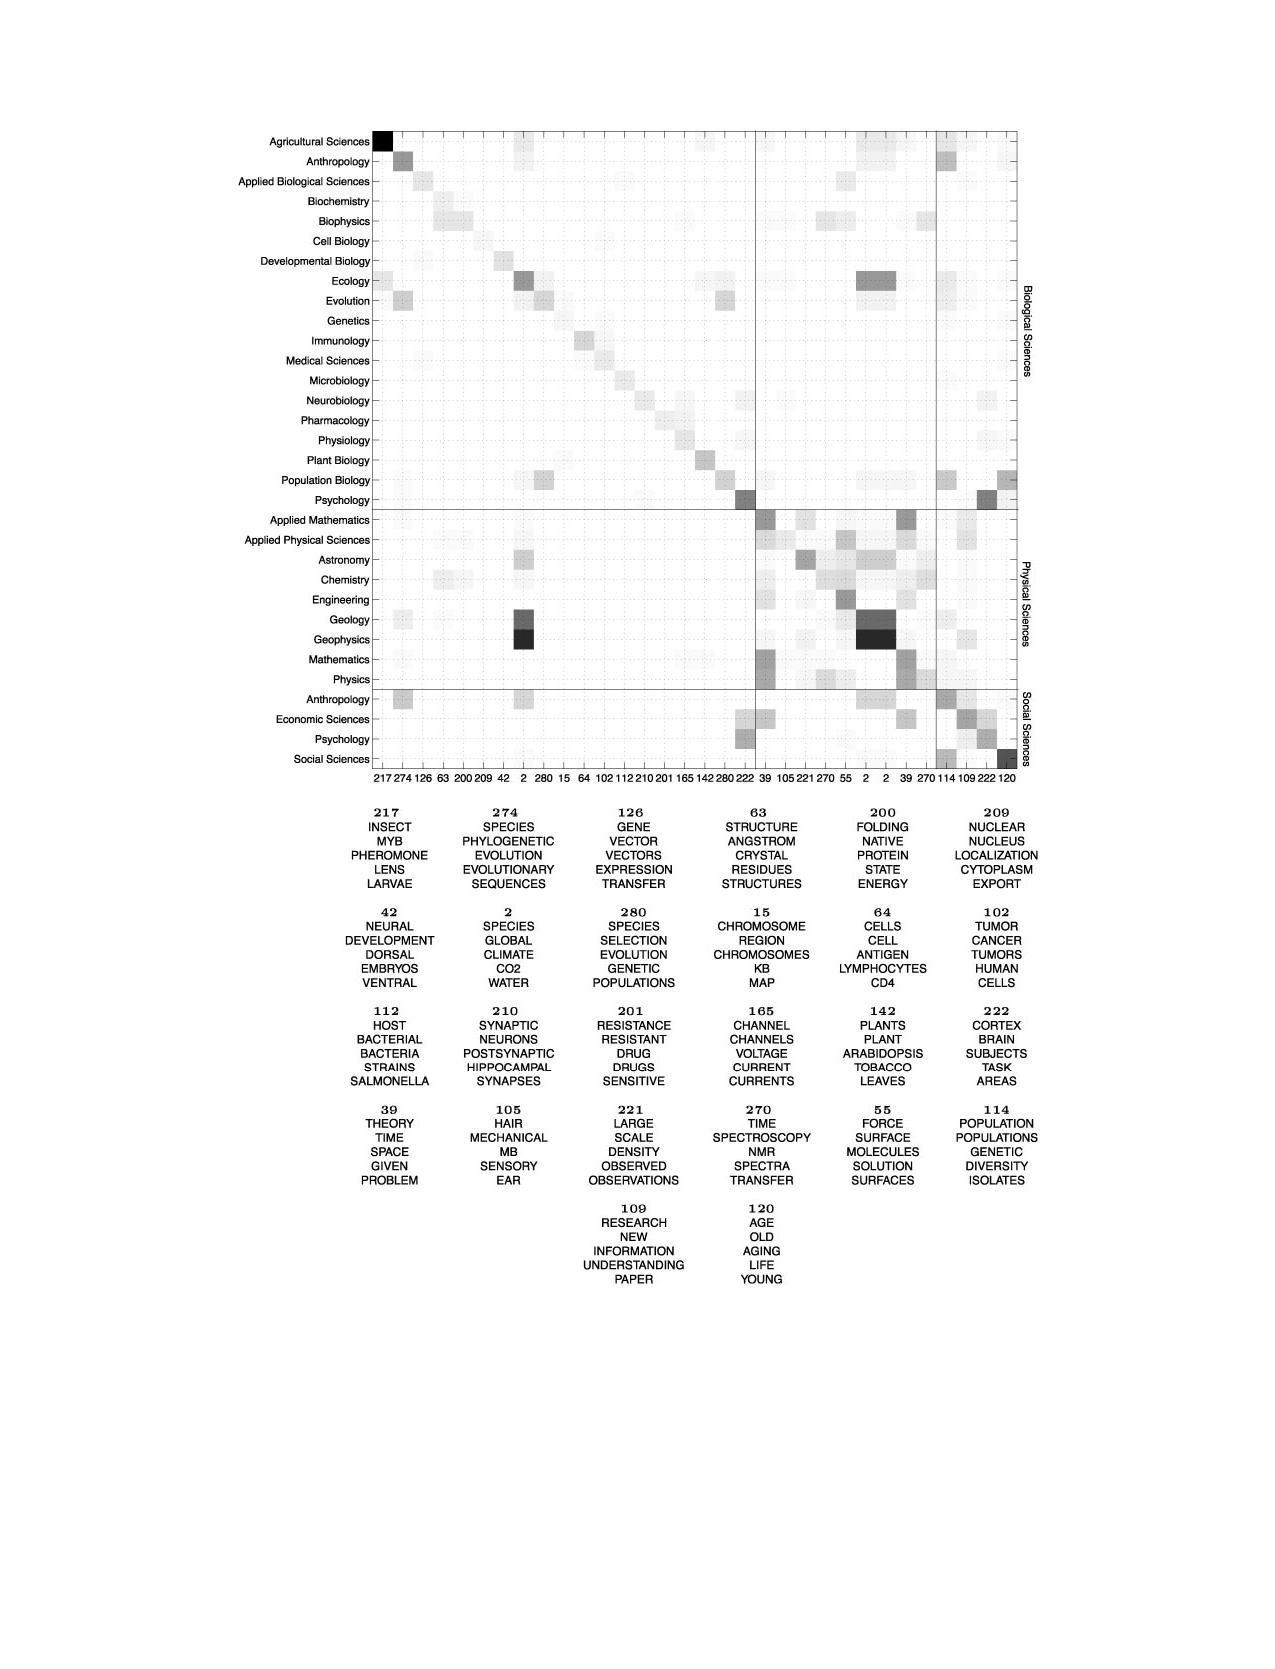
\includegraphics[width=.8\linewidth]{figures/sci_gs}
  \caption{After running a topic model on \abr{pnas},
    \citet{griffiths-04} found topics ($x$-axis) that could recreate
    the manually defined fields of study covered by \abr{pnas}
    ($y$-axis).}
\label{fig:pnas}
\end{figure}

One of the first uses of topic models was to understand the ``fields
of science''.  \citet{griffiths-04} found that they were able to
reconstruct the official \abr{pnas} topic codes automatically using
topic models (Figure~\ref{fig:pnas}).  This is a useful sanity check:
yes, topic models correlate with what we often think of as scientific
disciplines.  They use distinct language for methods, subjects of
study, and have different key players.

This work sought to find divisions between the fields of science, but from a retrospective point of view. 
In contrast, \citet{talley-11} sought to map the funding priorities of the American National Institutes
of Health (\abr{nih}) from within the organization.

The National Institutes of Health are America's premiere funding
agency for biological and health research.  The \abr{nih} consists of
several institutes that focus on particular diseases, research techniques, or body
systems; each of these institutes manages its own independent funding portfolio,
sometimes making it difficult to understand the ``big figure'' of funding.

\citet{talley-11} used topic models to help create this big picture,
in contrast to more labor-intensive techniques (e.g., keywords from a
meticulously organized ontology).  Their analysis discovered
unexpected overlaps in research priorities across institutes.  For
example, many institutes study angiogenesis, the formation of new
blood vessels; as a treatment for cancer, in heart imaging, the
molecular basis of angiogenesis in the eye, and how angiogenesis might
signal complications in diabetes.

In practice, applying topic modeling to the NIH grant abstracts collection was not straightforward.
Creating models that were acceptable to users accustomed to manually applied keywords required extensive curation of the vocabulary.
Topic models try to find topics to explain all aspects of a training corpus.
A collection of research proposals will have significant discourse related to non-research themes, represented by words such as ``propose,'' ``support,'' and ``funding''.
Large numbers of corpus-specific stopwords were identified for removal, mainly associated with the non-research topics.
In addition, \citet{talley-11} found that preprocessing documents to combine an extensive list of multi-word terms into single tokens made a substantial difference.
Scientific and other technical vocabulary often forms non-compositional compound terms because of the need for specificity.
As an example, ``amino acid'' contains the word ``acid'', but amino acids have no functional similarity to ``fatty acid'' or ``hydrochloric acid''.
Combining such terms into single-token compounds resulted in substantially improved specificity and comprehensibility in topics.

\section{How Fields Change over Time}
\label{sec:sci_change}

One way that science is distinct from the fields discussed in the
previous chapters in that scientists see themselves as building a single coherent structure of knowledge.  Each
paper in its own way stands on the shoulders of giants. Topic models
for science thus need to be aware of the connections between documents
over time.  Another way that science is different is that the
documents themselves introduce new ideas (we discuss detecting these
innovative ideas in the next section).

One of the first techniques to do this viewed topics as subtly
changing each year with a Dynamic Topic
Model~\citep[\abr{dtm}]{blei-06b}.  Each topic has a distinct 
distribution over words for each time period.  For example, the probability that
the \underline{physics} topic emits the word ``string'' in 1910 might be low, 
but after 1970 much higher.  Of course, we do not want the topics to be completely
different every year---we want topics to change, but not \emph{too
  much}.

The \abr{dtm} views topics as changing through \emph{Brownian
  motion}: the topic at year $t$ is drawn from a Gaussian distribution
with mean at the topic for year $t-1$ (a separate variance parameter
controls how much topics can vary each year).  At this point, you may
object given our discussion of distributions from
Chapter~\ref{sec:intro_building_blocks}: Gaussians produce continuous
observations that might be negative or greater than 1.0, while topics are multinomial distributions over discrete outcomes.

To move from Gaussian draws from $\vec x \in \R^d$ to a discrete distributions
over $d$ outcomes, \citet{blei-06b} use the logistic normal form to
create multinomial distribution
\begin{equation}
p(w=k \g \vec x)  = \frac{\exp{x_k}}{\sum_i \exp{x_i}},
\end{equation}
rather than drawing the multinomial from a Dirichlet distribution
(c.f. Equation~\ref{eq:phi_map}).
This greatly complicates inference, but allows the topics to change
gradually from year to year.

With this model, the \abr{dtm} discovers how fields change over
time.  At the start of the twentieth century, the language of
\underline{physics} focused on understanding how the ``ether''
propagates waves and the fundamental forces; by midcentury,
understanding ``quantum'' effects took precedence; by the end of the
century, experimental physics with large particle accelerators lead
the search for ever more exotic members of the subatomic menagerie.
While the final topic is nearly unrecognizable given the first, they
all are clearly \underline{physics}; the modeling assumptions of the
\abr{dtm} capture these nearly imperceptible changes in each year.

The flipping of a calendar page does not rule science, however;
changes can happen at any time.  \citet{wang-08} captures changes in
topics in continuous time; each document gets its ``own'' view of a
topic that can change slightly from the previous version of a topic.
This can help capture sudden changes in scientific topics, e.g. from
an innovative contribution.

% Author-topic model?

\section{Innovation}

The changes to fields happen because of \emph{innovation}.  Scientists develop
new techniques, new terminologies, and new understanding of the world.  These
concepts require new words which are reflected in their scientific
publications.  Unlike other fields, where documents merely report the changing
world, scientific documents are themselves the force that can change the world:
from Darwin's \textit{Origin of Species} to Einstein's papers on relativity.

Thus, it is interesting to try to find out where this change is happening.  From
a historical perspective, we might want to know who introduced
groundbreaking research first.  Measuring the context of innovations may also be useful for policy makers~\citep{largent-12}. 
Rather than awaiting ``magic'' or serendipitous findings, we might want to measure 
how conditions, teams, and forms of research collaboration lead to breakthroughs.
Better predictive models could then help direct new initiatives to recreate the settings that lead to important findings.

From a topic perspective, assessing impact amounts to detecting \emph{who} was responsible
for changing topics.
\citet{mann-06} find highly cited papers within the context of individual topics.
This approach helps to contextualize impact relative to sub-domains: a massively influential paper in mathematics may have the same number of citations as a moderately successful paper in molecular biology simply because the latter field is much larger.
They also search for papers that have topically diverse impact by measuring the topic entropy of papers that cite a given paper.
These broadly impactful papers tend to be methods and tools.
From an institutional perspective, \citet{ramage-10} take
a \textit{post hoc} perspective: after fitting a standard \abr{lda} topic model,
find the distribution over research topics in the entire research community at
time $t$ and then look back at time $t-1$ at the places who look like the
future.  They hypothesis is that these institutions ``lead'' other institutions to adopt
their ideas. % For example, they found that
% TODO: Add example!

Capturing more nuanced effects at either the individual or lab level requires
refining the model.  \citet{gerrish-10} adapt the random walk model of
\citet{wang-08} for scientific change.  Instead of topic randomly wandering into
new concepts, \citet{gerrish-10} propose that innovative articles ``nudge'' topics
to look more like them in the future.  This model is called the ``Dynamic
Influence Model'' (\abr{dim}). The assumption is that concepts and ideas are represented
by language. If we can identify changes in word usage, this change implies that there
were underlying changes in concepts.

For example, the Penn Treebank~\citep{marcus-93} revolutionized natural language
process and helped enable the statistical revolution in computational
linguistics.  Among its many effects is that people started using the word
``treebank'' much more than they had in the past.  \abr{dim} captures this by
explicitly modeling the influence $l_{k,d}$ of a document $d$ in topic
$k$.

% TODO: make notation consistent with paper and rest of this survey
Documents that do not make a splash have no measurable influence, while influential
documents are absorbed by other scientists, who adopt the influential ideas and, critically, their language.  Most documents will not move topics
at all so it is reasonable to assume that $l_{d,k}$ is zero for most
documents.  However, influential documents will change a topic.

A topic is changed by an influential document by making the topic's
distribution over words look more like the words in the influential document.  For example, the article
introducing the Penn Treebank uses ``treebank'' much more than
``potato'', so the topic will have a higher probability for
``treebank'' after incorporating a document's influence.

This incorporation happens similar to the drift of the dynamic topic
model (\abr{dtm}, Chapter~\ref{sec:sci_change}).  Instead of drifting
randomly, the \emph{direction} of topic change is based on the words
used in influential documents and the \emph{magnitude} of the drift is
how influential a document is.

Each of these terms are random variables; inference in the model discovers the
settings of the random variables that best explain the data.  The \abr{dim}'s
estimates of influence correlate well with the number of citations an article
gets (the traditional measure of influence).  Unlike citations, however, the
\abr{dim} can be used in more informal settings to detect influential
documents: for example, when a blog or a letter introduces influential
ideas.

While science communication is ostensibly about promoting ideas and new
understanding, topic models can also help understand less objective
communications where influence is not just about facts but also is about emotion,
beliefs, and relationships.  The next chapter discusses how topic models can
understand these messy, interesting properties of text.
